\section{Recurrent modules and task-dependent allocation}
\label{sec:modularsupp}

\subsection{Exact variance accounting with internal recurrence}

For stable real matrices \(A,D\) and fixed \(B\), write the
generator in output--source order. Its propagator is
\begin{equation}
 J_m=\begin{pmatrix}D&mB\\0&A\end{pmatrix},\qquad
 e^{J_m t}=\begin{pmatrix}e^{Dt}&mH(t)\\0&e^{At}\end{pmatrix},
 \quad H(t)=\int_0^t e^{D(t-u)}B e^{Au}\dd u.
 \label{eq:modularprop}
\end{equation}
Let the independent white drives have block covariance
\(\operatorname{diag}(Q_o,Q_s)\). The source variance is independent
of \(m\), and the output variance is the sum of independent local
and propagated contributions. Taking the trace in fixed physical
coordinates gives
\begin{equation}
 C(J_m)-C(J_0)=m^2\kappa,\qquad
 \kappa=\int_0^\infty\Tr[H(t)Q_s H(t)^\top]\dd t.
 \label{eq:modularcost}
\end{equation}
The integral is finite by stability. We require \(\kappa>0\)
for a nondegenerate price. Internal recurrence does not create
higher powers of \(m\), because no trajectory crosses the adjustable
intermodule coupling twice. This does not contradict the
square-zero truncation statement in Sec.~\ref{sec:cost}: that
statement scales the entire nilpotent coupling, whereas here
the recurrent internal matrices are fixed and only the
intermodule gain is varied. Cross-module return or correlated
source--output drive can destroy this separation.

A cue shifts the source initial state by \(\pm b\), independently
of stationary background fluctuations. For a fixed output vector
\(c\) and normalized temporal weight \(w_T\), the mean per unit
coupling is \(h=\int_0^\infty w_T(t)c^\top H(t)b\dd t\).
Let \(L\) be the readout variance from output-local noise alone
and \(S\) that from propagated source noise at \(m=1\).
Then \(z\mid\pm\) is Gaussian with means \(\pm mh\) and common
variance \(L+m^2S\). For \(L,S>0\) and \(h\ne0\),
\[
 d'^2=\frac{4m^2h^2}{L+m^2S}
     =\frac{4h^2}{S}\frac{x}{x+\kappa L/S},\qquad x=\kappa m^2.
\]
For a target squared discrimination \(0<y<F=4h^2/S\), the
minimum cost is \(x(y)=C_*y/(F-y)\), with \(C_*=\kappa L/S\).
An independent stationary Gaussian colored local process may
replace the local white drive, including through stable auxiliary
states; the separation and readout law hold with its actual
\(L\). A colored source requires its own propagated variance
and price, not the white-source value of \(\kappa\).

\subsection{General local-noise covariance: endpoints and crossings}

Let the two readouts share the same nonzero \(h(T)\), positive
\(S(T)\) and \(\kappa\). Comparing
\(F x_i/(x_i+C_{*,i})\) cancels their common ceiling, giving
\(d_1'>d_2'\) exactly when \(x_1/x_2>L_1/L_2\).
For real stationary local processes with continuous, absolutely
integrable autocovariances \(R_i\), assume \(R_i(0)>0\) and
\(P_i(0)=\int R_i>0\). Extend \(w\ge0\) by zero to negative
time and require \(w\in L^1\cap L^2\), \(\int w=1\). Then
\[
 L_i(T)=\int\!\!\int w(u)w(v)R_i(T(u-v))\dd u\dd v.
\]
Since \(|R_i(\tau)|\le R_i(0)\), dominated convergence gives
\(L_i(T)\to R_i(0)\) as \(T\to0\). For the other limit,
\[
 T L_i(T)=\int_{-\infty}^{\infty}R_i(s)
                   \langle w,w(\cdot+s/T)\rangle_{L^2}\dd s
       \longrightarrow P_i(0)\|w\|_2^2.
\]
Translation continuity in \(L^2\) and the bound
\(|\langle w,w(\cdot+s/T)\rangle|\le\|w\|_2^2\)
justify the limit. The same assumptions give continuity at
positive \(T\). If the fixed budget ratio lies strictly between
the endpoint noise ratios, there are finite short and long
durations with opposite rankings, hence at least one crossing.
This is a sufficient test; it is not necessary when the ratio
is nonmonotone, nor does it guarantee uniqueness. It compares
common attainable targets separately at each duration, not a
fixed target at every duration. Shared ceilings, source noise and
price coefficients are assumptions of the controlled comparison;
arbitrary recurrent modules need not satisfy them.

The main text's noise examples use
\(R_2(u)=0.25e^{-2|u|}\) and four choices for \(R_1\):
\(e^{-0.5|u|}\),
\(0.6e^{-0.25|u|}+0.4e^{-|u|}\),
\(0.85e^{-0.3|u|}+0.15e^{-0.7|u|}\cos(1.8u)\), and
the control \(e^{-2|u|}\). Their short-window ratios are all
four; the long-window ratios are respectively \(16\), \(22.4\),
approximately \(22.89\), and four. Each is a valid stationary
Gaussian covariance, realized by independent OU or damped
two-dimensional rotating components. Signal and propagated noise
are kept common, and the budget ratio is \(6.76\). Additional
noise-only output states can realize these local covariances
without modifying the common signal channel or its coupling price.
The examples are covariance-based checks, not anatomically fitted
circuits. Analytic boxcar integration is checked by direct quadrature.

\subsection{Two allocation objectives and their global solutions}

Assume independent pathways with separately adjustable forward
gains and no additional gain caps. Fix all internal matrices,
drive covariances, cue vectors, readout vectors and temporal
weights. Let \(F_i,C_{*,i},p_i>0\) and \(B>0\). Then
\(f_i(x)=F_i x/(x+C_{*,i})\) is increasing and strictly concave:
\[
 f_i'(x)=\frac{F_iC_{*,i}}{(x+C_{*,i})^2},\qquad
 f_i''(x)=-\frac{2F_iC_{*,i}}{(x+C_{*,i})^3}<0.
\]
The feasible simplex is compact, so maximizing
\(\sum_i p_i f_i(x_i)\) has a unique optimum. Monotonicity
uses all the budget. The KKT conditions give the main text's
allocation formula, with a positive \(\lambda\) uniquely fixed
by the budget. Zero allocations obey
\(p_iF_i/C_{*,i}\le\lambda\); funded pathways have equal
weighted marginal returns. These are standard separable concave
optimization conditions~\cite{boyd2004convex}.
For the active set \(\mathcal A\), the optimal utility is
\begin{equation}
 U^*(B,T)=\sum_{i\in\mathcal A}p_iF_i
  -\frac{\left(\sum_{i\in\mathcal A}
                     \sqrt{p_iF_iC_{*,i}}\right)^2}
         {B+\sum_{i\in\mathcal A}C_{*,i}}.
\end{equation}
The active set must satisfy the zero-allocation inequalities;
the all-active formula cannot be used below its activation thresholds.
When the cue sign is common but noise is independent across
pathways, the Gaussian readouts are conditionally independent and
the squared joint separation is the sum of the squared scalar
separations. Task weights other than one define a weighted
utility, not this unweighted joint decoder.

For the worst-output objective, a target \(y<\min_i F_i\)
requires at least \(\sum_i C_{*,i}y/(F_i-y)\) budget. This sum
is continuous and strictly increasing from zero to infinity.
Its unique root at \(B\) determines the optimum, and every output
attains the same squared separation. Common ceilings reduce the
root to the closed form in the main text. For two such outputs,
equality of the scores is equivalent to
\(x_1/x_2=C_{*,1}/C_{*,2}\), precisely the unique max--min
allocation at that total budget. Equality alone is not a claim
that a temporal sign change always occurs; the OU boxcar example
has that sign change by the monotonicity proved in Sec.~\ref{sec:crosssupp}.
Changing gains in this optimization preserves total cost and
the block-triangular decay spectrum, not in general the stationary
covariance eigenvalues.

\subsection{Independent checks and a temporal decoder control}

We generated 24 fixed stable module pairs, with source and output
dimensions between two and five, using random seed 271828.
Each internal matrix has dense off-diagonal entries and a diagonal
leak exceeding its absolute row sum by a positive margin, ensuring
stability. Half use positive and half signed off-diagonal entries;
both have recurrent cycles. The cross-module matrix is fixed and
Frobenius-normalized; diagonal drive variances are positive. For
each module, gains \(0.05,0.2,0.8,2,4\) and windows \(0.35,1.6\)
give 240 checks against the full generator. Stationary covariance
comes from a Lyapunov solve. Mean and window covariance are
integrated with matrix-exponential identities, with independent
48-node quadrature at unit gain for every module and duration.
The maximum relative discrepancies in cost and the readout law
are both below \(1.1\times10^{-12}\)
[Fig.~\ref{fig:allocationchecks}(a)]. These are numerical checks
of the exact derivation, not samples supporting a biological prevalence.

For the allocation rule, 36 seeded problems span two, four and
eight pathways with unequal positive ceilings, prices and task
weights. A constrained SLSQP solve independently checks the
analytic KKT objective; the max--min solution also checks budget
use and equal attained scores. The original two-pair example
is evaluated without changing its cue, noise or total budget.

Finally, we compare three temporal readers of the original
fixed-allocation example over \(0.15\le T\le5\). Sample each
output, including the cue-onset value, at maximum interval
\(0.01\). For sample means \(\mu\) and stationary covariance
matrix \(K\), any weight vector \(w\) has
\(d'^2=4(w^\top\mu)^2/(w^\top K w)\).
Uniform point weights approximate the boxcar; signal-matched
weights are proportional to \(\mu\). The optimal temporal
weights \(K^{-1}\mu\) give \(4\mu^\top K^{-1}\mu\).
They may be signed and are not constrained to resemble an
integrating downstream neuron. The covariance is evaluated from
the exact pair lag covariance, not fitted to simulated trials.
Halving the maximum interval from \(0.02\) to \(0.01\) changes
the slow/fast optimal-decoder ratio by less than
\(4.4\times10^{-5}\) relatively over the tested grid.

Uniform and signal-matched weights retain a ranking crossing,
but the covariance-optimal decoder does not: its smallest
slow/fast ratio is \(1.495\) [Fig.~\ref{fig:allocationchecks}(b)].
This is a benchmark on sampled finite trajectories, not a proof
of convergence to a continuous-time or infinite-horizon decoder.
It shows why fixed temporal integration is part of the
computational question. The allocation theorem holds for
prescribed temporal weights; optimizing those weights again
at every gain is a different feasible set.

\begin{figure}[t]
 \centering
 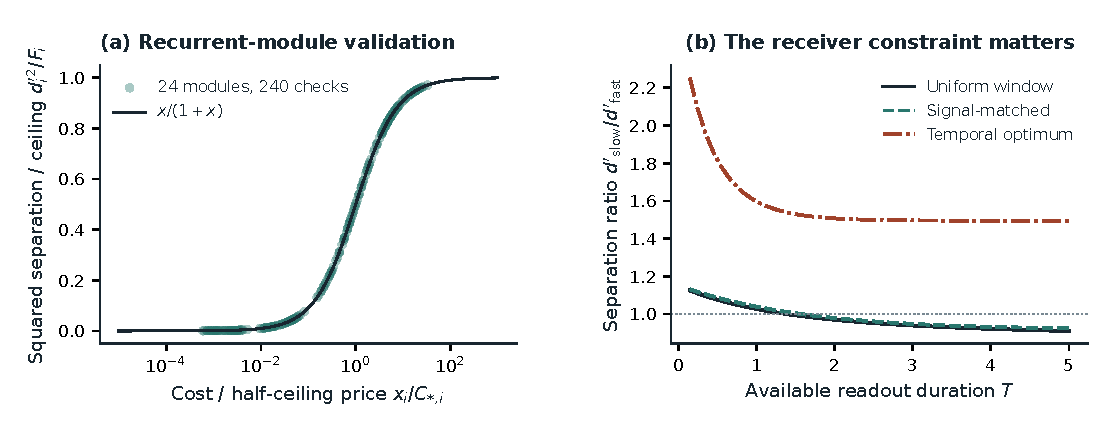
\includegraphics[width=\textwidth]{figures/fig_prrS_allocation_checks.pdf}
 \caption{\textbf{Generality checks and an unconstrained-reader benchmark.}
 (a) The 240 full state-space calculations for 24 recurrent
 module pairs collapse onto the normalized readout-cost law.
 The solid line is \(x/(1+x)\), not a fitted curve.
 (b) Ratios for the original two-pair example with uniform,
 signal-matched and covariance-optimal temporal weights. Only
 the last is allowed arbitrary signed weights adapted to the
 sample covariance. A ratio above one favors the slow output.
 Sampling intervals and model time units are specified in the text.}
 \label{fig:allocationchecks}
\end{figure}
